\documentclass{article}

\usepackage[utf8]{inputenc}
\usepackage[margin=2cm]{geometry}
\usepackage{multicol}
\usepackage{color}
\usepackage{float}
\usepackage{graphicx}
\usepackage{natbib}
\usepackage{hyperref}
%\usepackage[hidelinks]{hyperref} % Use this to hide boxes around links/refs
\usepackage{pdfpages}
\graphicspath{{images/navigation/}{images/app/}{images/overview/}}

\title{Software Design Study Report}
\author{A-Team}

\begin{document}
\maketitle

%\begin{multicols}{2}
\begin{abstract}
  Cars are ubiquitous in our modern lifestyles, unfortunately, the software systems in them do not keep up with other computing systems that we use. In this report, we aim to show how we tackled the problems and areas for improvement that we found in current car systems. Five areas of a modern car's feature set were focused on weekly, these being; the dashboard, media, navigation, safety and an accompanying smartphone app.
\end{abstract}

\section*{Introduction}
For years car companies have invested relatively little into their car's information systems and technological abilities. Inbuilt Sat Nav systems are often hard to use, update and are counter-intuitive. Since car companies are slow to adopt new technologies, even features that would have been possible many many years ago have not been widely used yet. For example, we still use the physical dials in the instrument cluster that we have used for years.

We have created an attractive and modern solution for digital technology in a car that we hope to see in future modern cars in production. In Section~\ref{sec:system-design} we will give explain the technical elements of our system design that can be found ranging from navigation to safety features. In Section~\ref{sec:nav} we will go into detail on the design process of our navigation system. In Section~\ref{sec:app} we will go into detail on the design process of our accompanying smartphone app.

\section{Overall system design}\label{sec:system-design}
\subsection{General}


\begin{itemize}
  \item Operating system
  \item How the system updates -- dual system architecture
  \item separate auxiliary system
 
\end{itemize}
\subsection{Algorithms}\label{ssec:algorithms}
\begin{itemize}
  \item Bidirectional A* Algorithm
    \begin{itemize}
      \item Heuristics
        % Talk about
    \end{itemize}
  \item K means algorithm --- grouping convoys
  \item Learning algorithm --- user preferences, Contextually Aware Routing etc
    % FIND A LEARNING ALGORITHM
  \item Safety Detection algorithms
    \begin{itemize}
      \item Head pose algorithm
      \item Tesla radar system?
      \item Recognising bikes --- trained from training images which are bikes with riders
        % This is if we are detecting bikes using this method of detecting bikes (we mentioned using the 360 degree vision from the cameras for seeing bikes)
    \end{itemize}
  \item Something for tiredness detection
\end{itemize}

\subsection{Storage}\label{ssec:storage} % Chris
Our design has three places that data will be stored, some data being temporary and some persistent. We will store information in the cloud, in the car's local SSD storage and on users of the app's smartphones.

The cloud will be used for the majority of storage, it is where persistent data will be synchronised to from the phone app and car. Storage for most data such as user profiles will be kept in an encrypted Oracle database. The cloud will store user profiles that contain details such as saved routes, privileges, seat preferences, dashboard layout, contacts and driver stats. The cloud will also store details about convoy groups, containing data on members, member locations, group messages, routes etc. Since the cloud hosts the API used by the car and app, other miscellaneous data will also be stored here such as software updates.

The car's internal SSD storage will be used for fast reading and writing of synchronised files and cached data primarily. Data queried from the cloud will be cached to grant a more seamless experience even when the car is not connected to the internet. Examples of cached data from the cloud include favourite routes, dashboard layout and seat positions. Since the centre console system is built around the Android platform, we have been able to easily allow certain apps from the Play Store. One example of an app that we would allow on the system is Spotify, for music playback. The Spotify app will be able to store all of its settings, cached data and offline playlists in the car's internal storage as well. Local music files synchronised from a home network will be stored in the car's internal storage. The dashcams will also record their video to the internal storage of the car, this will be limited to a default percentage of the drive's capacity (SSD can be upgraded) and recordings will overwrite old footage in order to reuse the assigned storage space. The basic version of the system will likely have at least 120GB of SSD storage, however, this could easily be upgraded by swapping out the drive from the glove box.
% * <frebib@gmail.com> 2017-03-22T12:19:33.906Z:
% 
% It's probably worth mentioning that the SSD can be user replaceable and as a result the system is stored on a separate disk(s) internally within the car to accommodate such feature
% 
% ^.

The accompanying car smartphone app does not require much storage at all since it must be connected to the internet or car to make any changes. Data from the cloud, car and app will be cached so that it may still be accessible for short connectivity outages.

\subsection{Data Structures}\label{ssec:data-structures} % Chris
In the system that we have designed, we require a few different data structures in order make our system efficient and easy to work with.

For our navigation algorithm, we decided to model the street map as a graph. Road junctions, route starting point and route destination are all represented as nodes in the graph, with roads being the edges that connect the nodes of the graph. This graph structure is most appropriate for us to use in our bidirectional A* search algorithm.

Routes will be kept in a JSON format with a JSON object containing two lists, one list containing nodes IDs of a route and the other containing the edge IDs. List items will be in chronological order for the route. The system is able to present the route on-screen by reading the lists to build the section of the street map graph that represents the route. This JSON format also allows for sections of the route to be updated easily by swapping out and adding nodes and edges. Another benefit of this format is that it is easy to implement the transferring of these routes from the app to the car.

The customisable dashboard layout will also be stored in a JSON format with widgets stored in a list object and more general details in a separate object. Widget objects in the list contain information about their relative position, size and styling in the dashboard.

User profile data such as username, route preferences etc.\ will all be kept in an encrypted Oracle database in the cloud, this will allow for us to have granular control over what information we receive when requesting user information.

An SQLite database will exist in the local storage of the car, this database will contain details of local music files that are also stored in the car's local storage. Music files that have been added to the car will have their song, album and artist names looked up and stored in the database. The SQLite database provides access to song details to the centre console and car app.

The smartphone app for the car system will use the same data structure for maps as the car uses. Cache data from the cloud and car will be stored in an SQLite database.

\subsection{User Accounts --- Matt}\label{ssec:user-accounts}
Something that we found is lacking across intelligent car systems in the market is the use of portable user profiles. By this we mean profiles that can be used across several cars, applying user settings and preferences where applicable.
There are several ways in which such data can be encapsulated and moved from car to car, including serving a database from a server to the car, transport via Bluetooth directly from a smartphone, use of NFC tags and many others.
\subsubsection{Storage and transport}
The method we found most suitable for doing this works by storing the data relative to each user profile online in an SQLite database and then serving it either directly to the car when a user logs in from in-car interfaces or to a smartphone application. Following this, the user is able to transfer the data to the car via Bluetooth with the press of a button. The data is cached on the phone and car, as applicable, to allow access even when internet access is limited or not available.
\subsubsection{Cardinality of accounts, vehicles and shared data}
Each user will have one account that will be able to contain multiple car profiles. Car profiles can share generic information, such as preferences regarding routing, music, favourite temperatures, speed dial contacts, etcetera if the user specifies so. Information specific to the car make and model, such as steering rack height, seat adjustments, wing mirror adjustments shall stay bonded to each car profile.
\begin{figure}[H]
  \centering
  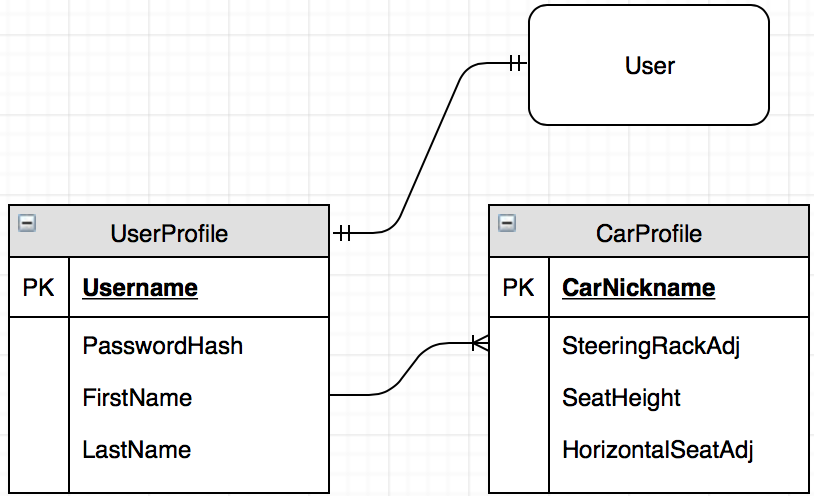
\includegraphics[scale=0.7]{profile-cardinality}
  \caption{Visualisation of cardinality of user profiles}\label{cardinality}
\end{figure}


\subsection{Communications \& Data Flows}\label{ssec:communications-data} %Tyler
Within our system, we have communications between the Mobile App, the Car and our Cloud, with links to external APIs.

\subsubsection{Communication between devices and cloud}\label{sssec:car-cloud}
The car and mobile app communicate with the cloud mainly to synchronise information. The device sends hashes and timestamps of their files to the server, which compares them with the latest versions. The files which are different are sent back to the devices for synchronisation.

Since the car and the mobile app can both change user profile settings, there will be continuous syncs when user settings or preferences are changed. This is so the user can change their settings away from their car with their phone, and have them set up automatically the next time they enter their car.

The software within our car has standard API requests that will always have a response from our cloud, we decided that the cloud would have a general API service, which would provide a link to the external APIs that we use. This is so we can provide the best API for a given location, and there is no unnecessary traffic going through our cloud. Also if external APIs are unavailable unexpectedly, we can always just update the cloud to provide a new link to a different external API. These services are mentioned in more detail in section \ref{sssec:devices-APIs}.

During navigation in convoys, the cars location is sent to the cloud and the associated group member's locations are pulled down from the cloud. This is so the location of other group members can be regularly updated on the navigation display. Other information such as group messages or navigation reroutes are also communicated between group members and the cloud.

All the system updates for the car's software will be downloaded through the cloud. These files will be verified using MD5/SHA1 hashes and comparing them to the hash provided by the cloud server. This is to ensure they are not corrupted or tampered with.

The cloud will always be listening for real time event data. This is the kind of events that would be happening live, such as if someone is breaking into your car or for some reason the car alarm has just gone off. Once in the cloud this information would be passed straight to the car owners phone via the app to alert them.

\subsubsection{Communication between car and phone}\label{sssec:car-phone}
Communications between the car and the phone consist of initial connection, instructions and data transfer. Establishing a connection is done by pairing the phone to the car by means of NFC, this will authenticate the phone with the car for communications over Bluetooth and Wi-Fi. Authentication can also be achieved by typical manual methods such as typing in a password. There will also be the standard Bluetooth communication between the phone and the car such as sharing contacts and taking calls.

Many features of the app communicate with the car, these features are described in Section \ref{ssec:app-tech} [\nameref{ssec:app-tech}]

\subsubsection{Communication between devices and external APIs} \label{sssec:devices-APIs}
Many sections of our system gather a lot of information from external APIs. This information ranges from data required for navigation to getting the latest weather forecasts.

While using navigation, the car will automatically get the latest information on roadworks, current traffic conditions and information on public transport. This information will be based on the location of the car and is used to add displays to the map. For example showing roadworks in locations where roadwork is occurring.

Our dashboard can contain widgets to display simple information like weather which would be pulled down from the cloud and updated regularly.

\subsection{Information Security}\label{ssec:information-security} % Joe
A major focus for any internet connected technology is security, and with our car systems it is no different- the last thing a customer would want is to have their car stolen by it being driven into the distance by a remote thief. We employ a model of `encryption everywhere' to ensure maximum data security, paired with very strong authentication to prevent unauthorised access or control. Security is a primary focus in every aspect of the car system, the following non-exhaustive list are some of our main focuses

\subsubsection{Data Communication}
Every connection that is made in our ecosystem leverages the flexibility and security of TLS for both encryption and authentication. TLS provides a strong suite of ciphers cross-compatible with any device. Industry standard hardening techniques are employed at both client and server end to ensure the strongest connection possible such as only using strong mutually-agreed cipher suites and key exchanges.

This widespread usage of full transport encryption is viable due to the hardware-accelerated AES-NI and similar instruction sets built into most modern CPUs by manufacturers like Intel, AMD and ARM* (dependent on model and chip manufacturer). Without hardware support, encryption would be very expensive in terms of computation for every device: servers, cars and most importantly mobile devices such as smartphones and embedded devices.

Performing AES or similar encryption purely in software is very slow and consumes a significant amount of CPU cycles and battery power resulting in a poor experience thus making encryption on lower power and mobile devices not at all feasible.

Another advantage of using TLS is `Perfect Forward Secrecy' of data when the appropriate key-exchange protocol is used such as a Diffe-Hellman based exchange method. This provides the guarantee that any data that is intercepted in transport by a 3rd party cannot decrypt the data with a previously apprehended pre-shared key or certificate as the short-lived session token has been lost.

\subsubsection{Data storage \& encryption}
{\Large\color{red} Decide data storage encryption}

\subsubsection{User Authentication}
We leverage the implicit authentication flow from TLS backed by per-user certificates (specification defined at \url{https://tools.ietf.org/html/rfc5246#appendix-F.1.1}) which is a security advantage to the cloud provider  as it is more secure authentication method than using a password and presents a cleaner user experience as it requires no input from the user whereas a password would do.

Everywhere a persistent login is used, it is replaced with a client certificate authorised to access the account without a password. The primary use for these certificates is automatic authorisation of the mobile app on smartphones and embedded devices with the cloud servers and the car. The certificate must be present for communications with a car and is preferred for authenticating with cloud servers as it provides significantly better security than a password and requires less interaction from the user.

For each additional device that a user adds to their account, a unique certificate is generated and stored on the device therefore allowing each user device to be tracked individually, linking the device to the specific user. 

Further discussed in Section \ref{ssec:app-security} [\nameref{ssec:app-security}] are additional security features used specifically within the mobile application for extra convenience and protection.

\subsubsection{Server and Car Authentication}
Similarly to user authentication with certificates, each car system has an in-built signed certificate from the car manufacturer to prove it's authenticity. The matching private key for the certificate is installed in a hardware keystore within the car computer to improve it's robustness against attacks and is communicated with over a standard bus built into the car computer system.

Unlike the mobile app, the car must always use it's certificate when communicating with any external service and can only communicate over the encrypted and authenticated HTTPS protocol. This is to ensure no future attacks are developed by exploiting the availability of unencrypted communications.
The car system will only handshake successfully with services that it recognises immediately, or those which have been signed by a recognised authority, as any HTTPS connection should.
Any system in the car that is not directly tied to critical or sensitive services may continue to use a standard CA (certificate authority) list; it is only internal services used directly by the car that require the manufacturer-trusted CA store.

The situation is very similar for the security implementation in the cloud. Each server is provisioned with a certificate/key pair, signed by the cloud provider and governing body, which are used to handshake every connection to the car and mobile app.
It is important that all endpoints communicating with these services ensure they check the validity and authenticity of the TLS certificates to prevent unwanted data leakage or MITM (man-in-the-middle) attacks where some critical authentication or identifying information could potentially be stolen. Any attacker posing as a rogue cloud server could forge certificates and assuming the client (whether that be an app, web client etc) doesn't verify it is signed by the correct authorities then the attacker can read all data passed to it unencrypted, as it was originally sent.

\subsubsection{Device Certificate Revocation}
Certificates can be revoked individually, on a per-device basis; this allows a user to instantaneously prevent any unauthorised access to the car(s) in the case a phone/laptop is lost or stolen. 

A user can revoke a certificate from their account at any time via the web portal or by calling the manufacturer's helpline, both of which are critical high-availability services as the security of vehicle control is paramount. Upon revocation, repeated push calls are made to every device on the account, including the car, to advise of the updated access  control. This is important as while many services are always authenticated through the cloud services like `remote access' of the vehicle (where revocation would immediately apply), some processes such as local unlocking via NFC or accessing the in-car computer only authenticate locally for speed and would have to be wait for the revocation update to be received. \textit{It should be very clearly noted that car ignition requires sufficient cloud authentication so the car cannot be started with any revoked certificate, ever.}

\subsubsection{}

\begin{itemize}
  \item Database encryption in the cloud
    % * <frebib@gmail.com> 2017-03-20T22:31:12.891Z:
    %
    % Is this a thing?
    % Maybe the data can use end-to-end encryption, only unlockable with a key from the user account?
    % ^ That however means the user is fleeced if they forget their password
    %
    % ^.
  \item HTTPS for all internet communications
  \item WPA2-PSK with AES for Wi-Fi hotspot login
\end{itemize}

\subsection{Interaction Design --- Matt}\label{ssec:interaction-design}
The interaction designs used on our product's interfaces were designed loosely based on designs from industry leading companies but tailored to integrate our ideas and implement some recurrent suggestions found throughout our research, which has seen over 100 responses. Our product requires three main interactive interfaces for users to effectively communicate with the in-car system:

\subsubsection{Centre console}\label{sssec:centre-console}
This is a 10 inch screen located in the middle section of the dashboard. Its purpose is that of displaying most of the information that flows through the car that may be of interest to the user and for the user to interact with it. For instance, destination input for the navigation system, joining and managing convoys, customising the instrument cluster, querying the system for detailed engine data and many more interactions will be performed on this device.

We found that in the recent years the integration of touch screens on dashboards has become a recurrent trend amongst major manufacturers and believe that it is an essential feature for the cars of the future due to how visible, versatile and aesthetically pleasing they are.

\subsubsection{Mobile app}\label{sssec:mobile-app}
As usage of mobile apps is constantly increasing, more and more industry leading companies are adopting this as a new mean of interaction with their automobiles. We firmly believe that this will become and essential feature to all cars within a few year and therefore have designed and prototyped one. More detail can be found in Section~\ref{sec:app}.

\subsubsection{Device on rear doors}\label{sssec:device-rear-doors}
Each of the rear door cards will be fitted with a 5 inch touch screen device that enables passengers in the rear of the car to search and add songs to the cars' shared music queue from different streaming services or a local library.

\subsection{Aesthetics/Graphical Design --- Matt}\label{ssec:aesthetics}
% User Interfaces of the above devices
An effort was made to follow current styling standards used in industry to give the user a familiar experience, therefore flat designs were used where possible. Also characterising our design are large icons and avoidance of large swathes of text.

\subsubsection{Dashboard cluster screen}\label{sssec:cluster-screen}
A screen will be replacing the usual instrument cluster behind the steering wheel. This will display information relative to speed, engine revolutions, fuel levels as it has been doing for the past decades but with the difference of being fully customisable in layout, content and colour. These features will result in improved user experience for individuals with poor vision and colour blindness since font sizes and colour schemes can be altered easily in the settings. More generally, as suggested by our questionnaire research, the majority of users will enjoy having the ability of selecting what they will see behind the steering wheel themselves. The LCD panel in question will not be a touch screen since access would be restricted by the wheel and the customisation will be managed on the centre console screen instead.

\subsubsection{Centre console}\label{sssec:centre-console-aestethics}


%%%%%%%%%%%%%%%%%%%%%
%	PLAN
%%%%%%%%%%%%%%%%%%%%%
\begin{itemize}
  \item Mobile phone
  \item Rear side door device
    % Justifications of why we have chosen these designs
\end{itemize}




%%%%%%%%%%%%%%
%
%	NAV
%
%%%%%%%%%%%%%%
\section{Feature 1: Navigation}\label{sec:nav}

\subsection{Research --- Lewis}\label{ssec:nav-research}
As part of the brainstorming process, we investigated current technology to see how the current navigation systems were perceived by various people. The first part of this research takes the form of a questionnaire we created to gain opinions on both current technology and some of our ideas. From this, we confirmed our beliefs that most people use their phone as their SatNav device; and are generally happy with current methods of controlling a SatNav, being touch screen and voice control. We also gained some insight into some design decisions to take, with a majority of survey participants being interested in seeing friends travelling with them; speed cameras; traffic; and road obstacles such as roadworks, accidents and breakdowns, on the map - while there was less interest in tracking emergency vehicles and breakdown recovery vehicles. There is also a high amount of interest in having various destination suggestions available to the driver. The survey  indicated to us that some features are already being executed well; most people find the directions given by their SatNav to be quite clear.
% Link to survey responses?

We also performed some research to find out exactly what kind of features are currently offered by SatNav systems. As part of this research, we discovered that a lot of our brainstorming ideas are already in development by some companies. A lot of these concepts are being produced by Google: if you search for a location on Google, there is an option to send the location to the maps app on your phone; your movements are analysed by Google to determine favourite places and routes.
% Probably more to say here...
During this research, however, we could not find any current implementation nor professional research into our ideas for convoy driving. The closest concept to this we could find was the Garmin Tracker
% Reference... not sure how we're doing references to external sources, yet. Also might be worth only referencing this lower down.
which seems to have very limited functionality for tracking a person who owns a Garmin SatNav, for uses such as knowing when a family member should reach home. It also appears that this feature is only included with a limited subset of the Garmin models, which seem to have been discontinued. \cite{RefWorks:2} 
% If we're going with Harvard referencing (must finish the reference if so)
mentions the existence of this tracker, stating ``this could be useful if you are in a big group and you have more than one car travelling to the same destination'', but does not elaborate further, and we cannot find documentation from Garmin as to whether this is the exact use of this tracker.
% Complete above paragraph? Might be finished now

\subsection{Brainstorming --- Matt}\label{ssec:nav-brainstorming}
% Should we include our initial ideas document?
In the first stage of our brainstorming we created a Google document which allowed us to collaboratively write down all the ideas we could come up with. By discussing them within our group, new ideas kept being generated and even different variations of the ideas we already had. In order to keep the design space as open as possible, during this stage, all ideas were noted down and considered, no matter how far fetched. Following the initial stage, and an iteration of research, we went through the document and filtered it, as a group, for the concepts that we wanted to take forward in our design. During the second stage of brainstorming we created a new document, containing only the chosen ideas to expand and research them in more depth.

An aid we found very useful was personas, a list of made-up personalities with realistic interests, jobs and attributes. During the brainstorming each of us tried to empathise with the different personas and think about their habits, things they enjoy, their mental states throughout different times of the day and from there, think of their needs, features they would enjoy and why.
% The personas are mentioned here, do we introduce them somewhere? Should it be in a research section or expanded upon here? -Lewis

Some of the ideas that came from our brainstorm are: Convoy tracking using K-Means clustering, public transport integration (including park and ride suggestions), route scheduling via either mobile app or in-car interfaces.

\subsection{Tech background --- Lewis}\label{ssec:nav-tech}
% Didn't realise how big this section might be, since there is a lot of technical detail in the slides for nav
\subsubsection{Routing algorithm}\label{sssec:nav-tech-routing}
The routing algorithm we use is bidirectional A* search, performing a typical A* search from the start node to the destination, and the destination to the start node, in parallel. The heuristic used for this search will incorporate:
route requirements;
% What are route requirements?
learnt user habits \& preferences, applying lower weight to road types preferred by the driver such as if they frequently divert through smaller roads, and applying a higher weight to road types that tend to be avoided by the driver;
roadwork and traffic information, gained from the APIs, which will apply a higher weight to roads based on their traffic levels.

In order to ensure the route continues being efficient, the system polls the APIs every five minutes for updates to traffic conditions and roadworks. After this data has updated the graph, the search is re-run, with the start node being ahead of the current position in order to account for the latency in running the search. The search also re-runs when the driver leaves the current route, to make sure they are still travelling efficiently.
\subsubsection{Machine learning}\label{sssec:nav-tech-machinelearning}
%
% I think Matt did some research into this? If so, can he fill out this section?
%
\subsubsection{K-means clustering}\label{sssec:nav-tech-kmeans}
One of the problems we encountered while designing the convoy feature was how to handle situations where a group is starting its journey separated, and quite widely spread. From our brainstorming sessions, we decided to implement k-means clustering as a method for grouping the members of a convoy together. As described in figure \ref{nav-kmeans}, any members of a convoy who wish to group together as quickly as possible to travel together on the main shared route will be grouped together through clustering. A number, $k$, (explained later) of ``means'' are randomly placed on the graph, and then two steps are repeated until the optimal positions for the means are found - determined by them not moving from the previous iteration. 

The first step is to create the clusters (step 2 of figure \ref{nav-kmeans}), associating each member of the convoy to their nearest mean. The second step moves each mean to the centroid of their corresponding cluster. When convergence is reached, the means are moved to the closest suitable waypoint on the underlying map, and each cluster of convoy members is routed to this waypoint in their cluster. When the entire group is starting within the same city, assuming the destination lies outside the city, this should be sufficient; however, as the convoy gets more spread, this algorithm becomes less efficient, since members may be travelling very far individually before they reach their cluster waypoint. The solution here is to iterate the algorithm multiple times, with the start nodes of each iteration being the cluster waypoints generated by the previous iteration, reducing $k$.

There are some further issues with this algorithm that need to be addressed. Firstly, a good value for $k$ should be chosen. This value represents how many clusters are created by the algorithm, and therefore the average number of people (or groups, if this is a later iteration) to be grouped together by a given iteration can also be determined from $k$. Therefore, $k$ should be chosen based on how many people should be grouped up during one iteration; the standard default will aim to group together 3 or 4
%
% Requires a choice and justification
%
people per iteration, meaning by default that $k=\frac{number\ of\ input\ nodes}{3}$. This may need to be changed or adapted based on the context, and can also be chosen by the convoy leader, where they can specify how many should group up per iteration; the leader can also specify to not use clustering, allowing each driver to decide how they reach the destination.

The second issue arises when this algorithm would introduce a large inconvenience for certain members. In figure \ref{nav-kmeans}, it can be seen that the topmost blue member of the convoy starts out close to the destination, but the algorithm forces them to travel in a different direction. When the algorithm detects that the clustering route is significantly longer than a standard individual route, it presents an option to that member to: accept the longer route, allowing them to group up with the others as quickly as possible; join directly into the full shared route, so they can still travel with the other members, but won't join up with them as quickly; or ignore the clustering, and follow an individual route, so they can reach the destination as quickly as possible while sacrificing the ability to travel in the main group.

\begin{figure}[H]
  \centering
  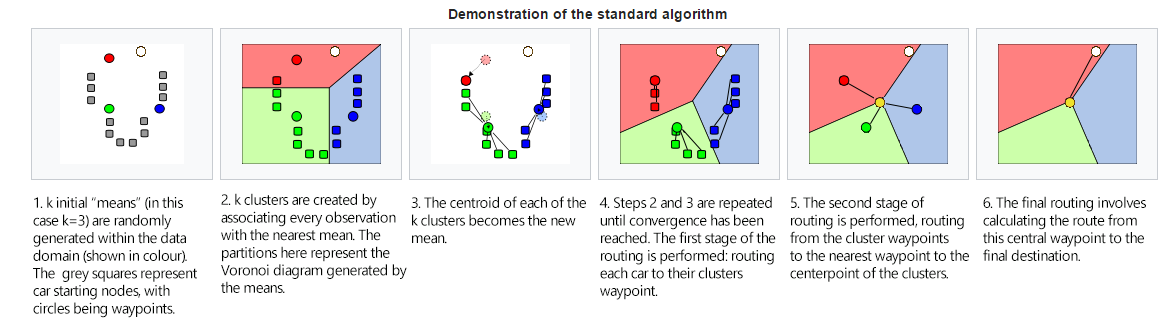
\includegraphics[scale=0.5]{kmeanscluster}
  \caption{Demonstration of K-means convoy clustering.}\label{nav-kmeans}
\end{figure}

\subsubsection{Public Transport}


\subsection{Convoy}\label{ssec:nav-convoy} % Chris
Convoys are a feature in our system, designed to allow a party to all route to the same destination, tracking members and having functionality for scheduled stops, rerouting and group calls. From the navigation menu, the user can select to either set up or join a convoy. The user that chooses to set up a convoy is given a six-digit code that they can then share via social media or any other way. Users that choose to join the convoy must enter the six digit code they were given by the convoy creator. The convoy creator is able to set the route destination, any stop off points and optionally give the convoy a name.

Once a convoy is set up, members of the convoy are able to see the shared route and coloured icons for members on the map. In the case that convoy members are starting their journey from different places, members will be grouped, with groups having different routes to a point of convergence. Like the normal navigation mode in our system, the route for an individual can be adjusted to re-route them back to the convoy in the case that they go the wrong way. Another feature of the convoy system is that it provides the ability to make group VoIP calls so that users can communicate hands-free, this is done using peer-to-peer technology over the car's internet connection (provided it has one).

Users may want to use convoys despite being far apart from each other, in this case, users may not be likely to arrive at similar times and so routes are individually calculated on each car's system and uploaded to the cloud. Each user follows their own route and can see the expected time of arrival for other members in a sidebar. Should two routes converge at any point, members will be moved onto a shared route when they reach that point, making meeting up more likely and reducing the number of routes to be stored in the cloud.

A convoy member can leave the convoy at any time, however, there are points at which the system will prompt them to leave the convoy. The first occasion for a prompt is when the current driver of the car changes, the new driver might be wanting to travel to somewhere else. The driver can, of course, cancel the prompt, this is useful for a situation where for example people share the responsibility of the driving for a long journey. Another time that a prompt to leave a convoy may occur is in the event that all convoy members have arrived at the destination, at this point, there will typically be no further use for the convoy. The final situation for a prompt to leave a convoy is if the car is inactive for 24 hours, users typically will not be resuming a group journey after such a long time.

Convoy data is collected and distributed to all convoy members from the cloud. The cars will download routes via the cloud API and send GPS location updates to the cloud every few seconds, these location updates will then be pinged to all other convoy members to keep the location of cars synchronised on all screens. Once the cloud receives a new location for a member, it immediately deletes the old, redundant location.

Limited functionality of the convoys feature is available through the app. Users with the app are able to set up or join a convoy, this data is synchronised to the cloud and then used by the car.

There are of course limitations to this feature. Convoys require an internet connection to update member locations. If any member fails to update their location, their icon will stay in place and fade away until a connection is regained and the location is updated once again.

\subsection{Design choices \& argumentation --- Lewis}\label{ssec:nav-design}
\subsubsection{General Design}\label{sssec:nav-design-general}
For a lot of features in our navigation section, we have utilised QOC as a method of deciding how to implement them. We have also used our survey responses as guidance for certain features.

We have employed a scoring system in the QOC in order to rank the options, which uses the importance levels of the criteria to determine how the options compare to each other.

\begin{figure}[H]
  \centering
  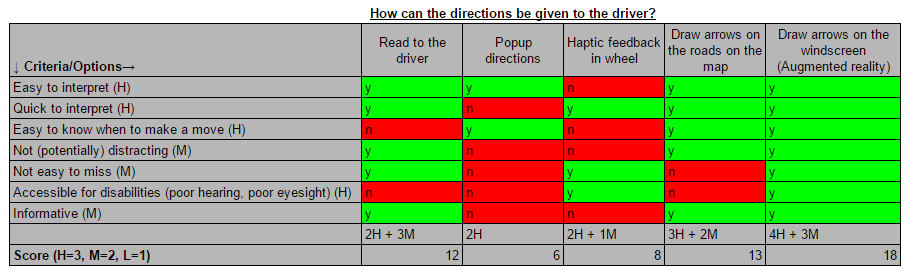
\includegraphics[scale=0.5]{qoc-nav-instruction}
  \caption{QOC discussing how to direct the driver}\label{qoc-instructions}
\end{figure}

Figure \ref{qoc-instructions} asks how directions can be given to the driver. As can be seen, an augmented reality approach appears to be a strongly decisive victor among these options, however, we had already discussed the ideas of augmented reality and head up display during the dashboard section of the design process, where we dismissed pursuing augmented reality for various reasons. For example, experiments conducted by \cite{RefWorks:3} 
conclude that "the driver's attention to the road and traffic is likely to be compromised" when HUD information is shown on the windshield. After some internal discussions we also feel that: it would be difficult to ensure it works in bright daylight and during nighttime; it would likely be expensive to implement and maintain, due to the high computational requirements as well as the cost of replacing projector bulbs; 

\begin{figure}[H]
  \centering
  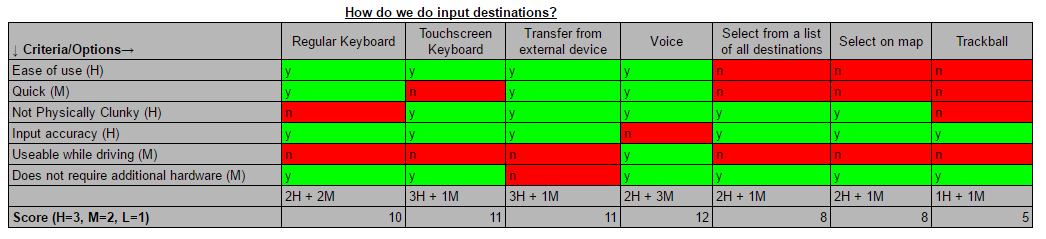
\includegraphics[scale=0.5]{qoc-nav-input}
  \caption{QOC discussing how to input a destination}\label{qoc-input}
\end{figure}

\begin{figure}[H]
  \centering
  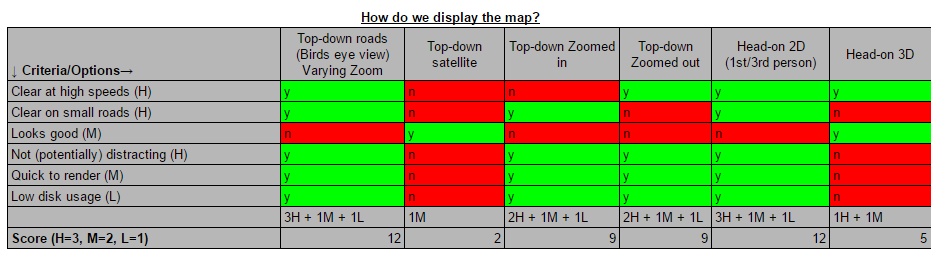
\includegraphics[scale=0.5]{qoc-nav-map}
  \caption{QOC discussing how to display the map}\label{qoc-map}
\end{figure}

\begin{figure}[H]
  \centering
  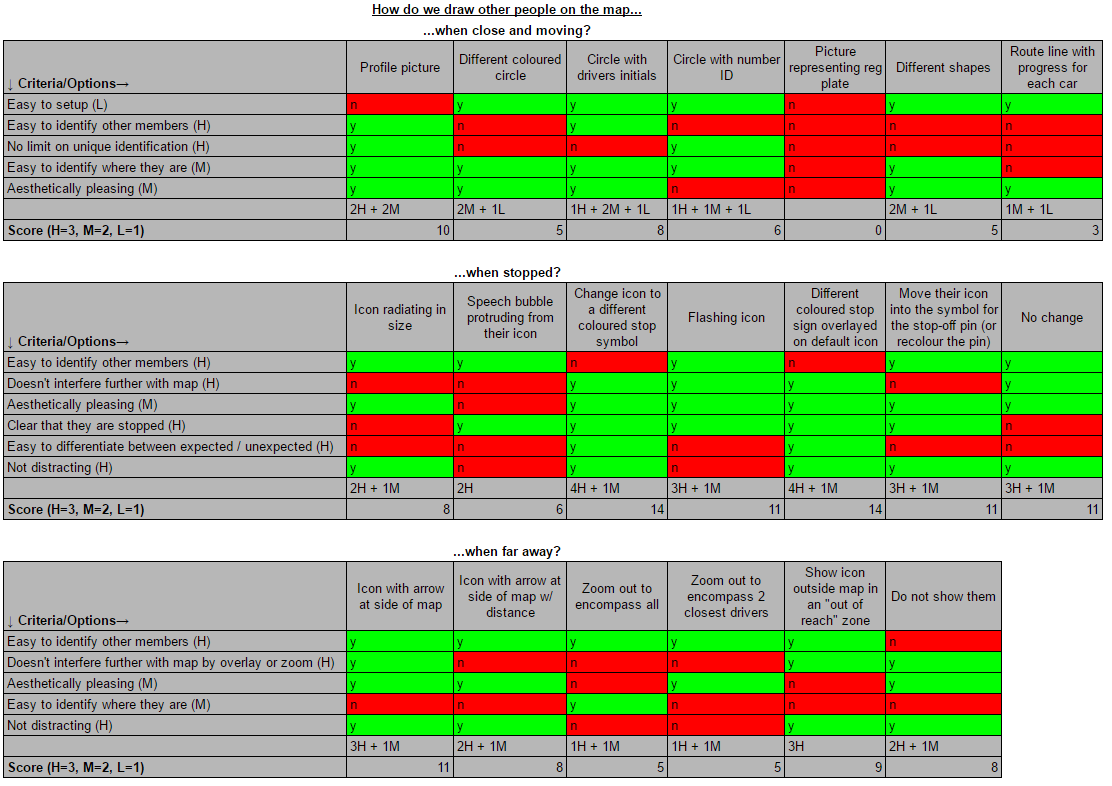
\includegraphics[scale=0.5]{qoc-convoy}
  \caption{QOC discussing how to display others in a convoy group}\label{qoc-convoy}
\end{figure}

\subsubsection{Algorithm justifications}\label{sssec:nav-design-alg}
% We don't really have much justification for k-means and we don't have much information in general about our machine learning
We used QOC as well as experimentation to determine which routing algorithm to use for navigation.


\begin{itemize}
  \item QOC % Some of the QOC matrices are incomplete or have incorrect scores
  \item Justification for algorithms
    \begin{itemize}
      \item Routing
      \item Clustering
      \item Contextually aware routing
    \end{itemize}
\end{itemize}

\subsection{Prototypes \& user testing}\label{ssec:nav-prototypes-testing}
\begin{itemize}
  \item Lo-Fi and Hi-Fi prototypes of Navigation and Convoy
\end{itemize}
\begin{figure}[H]
  \centering
  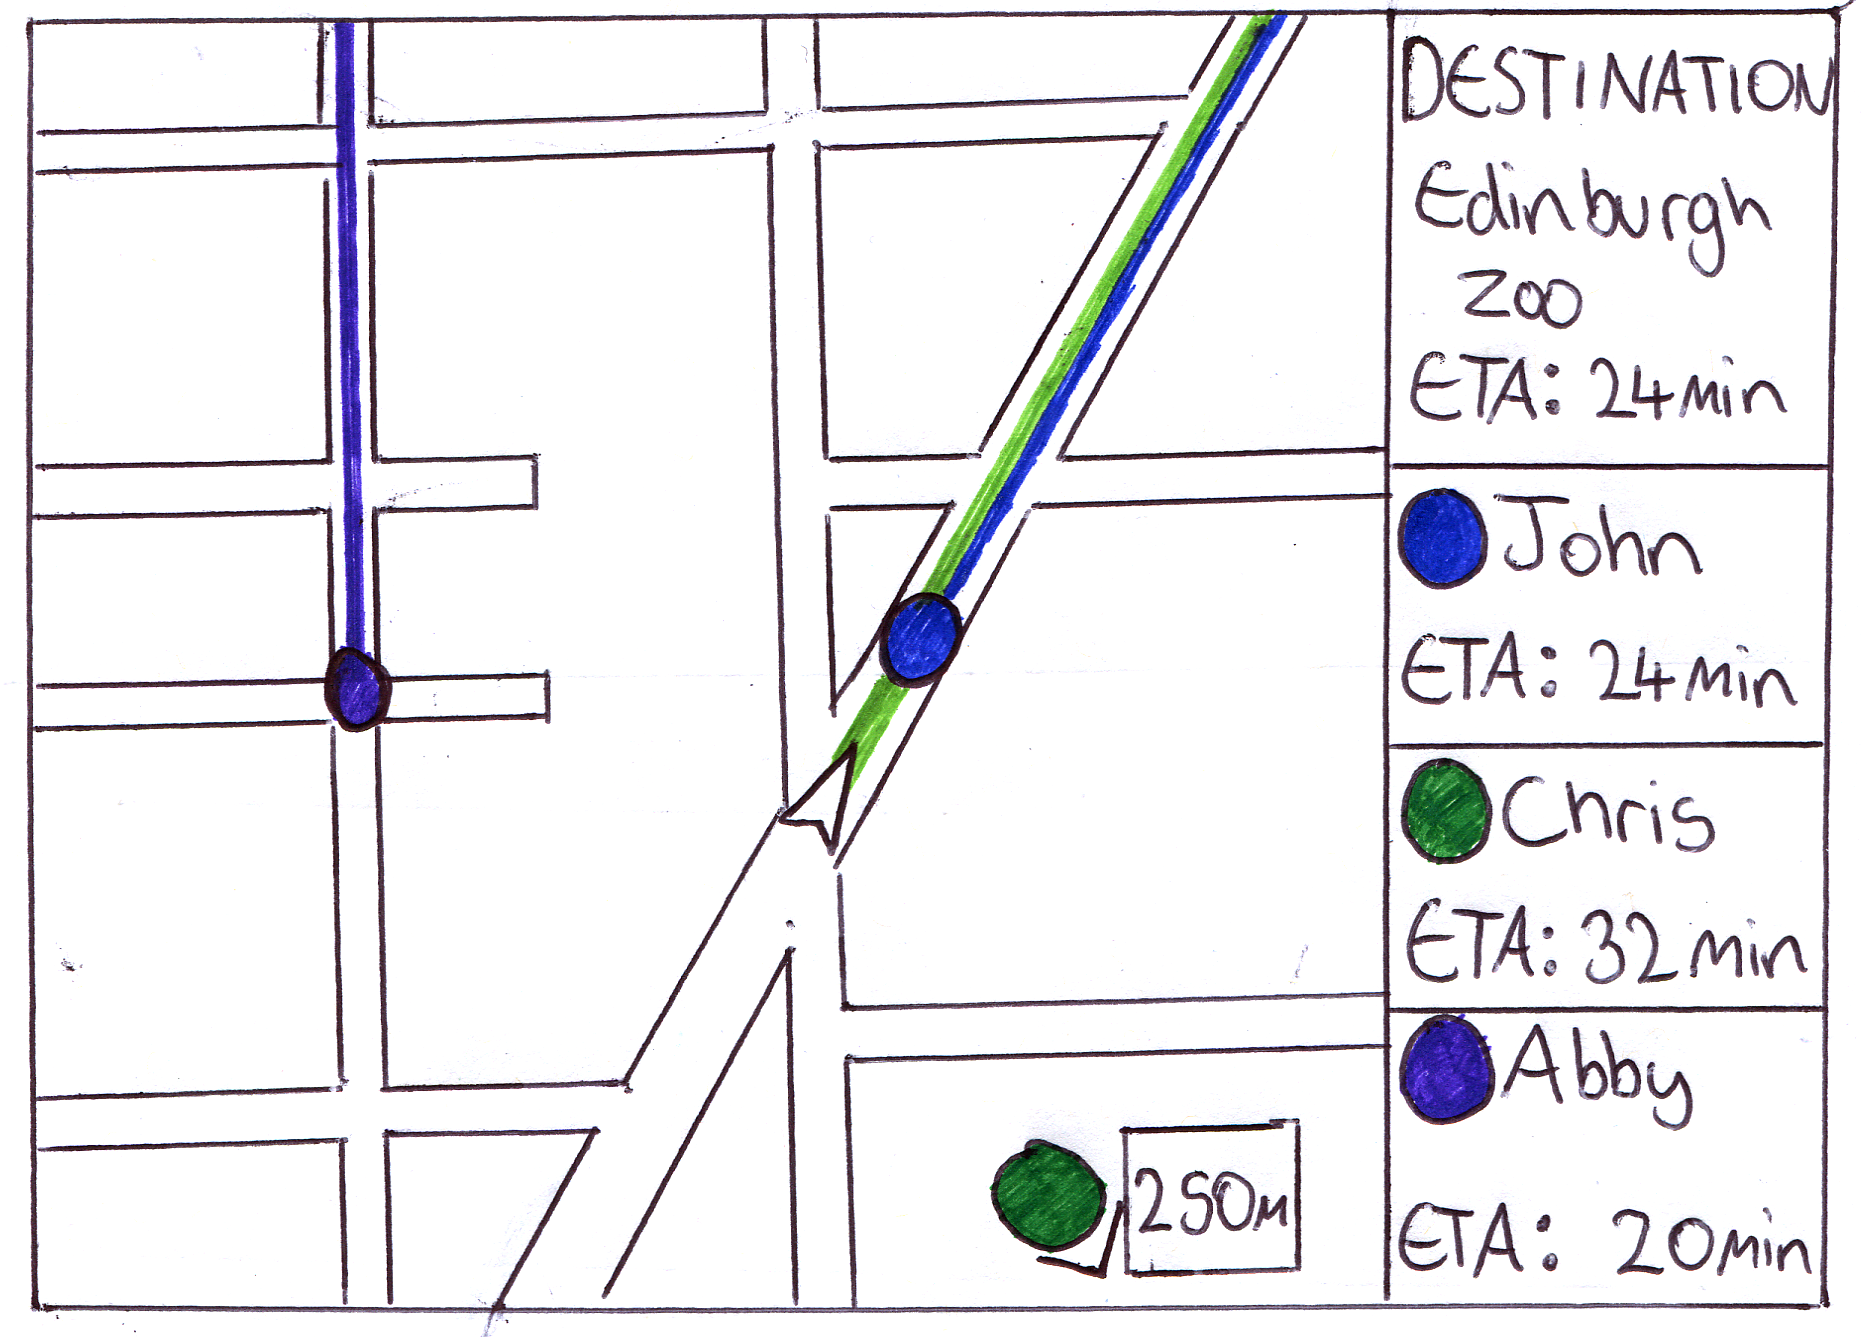
\includegraphics[scale=0.5]{convoy-lofi}
  \caption{Lo-Fi design for travelling different routes in a convoy}\label{prototype-lofi-convoy}
\end{figure}

\begin{figure}[H]
  \centering
  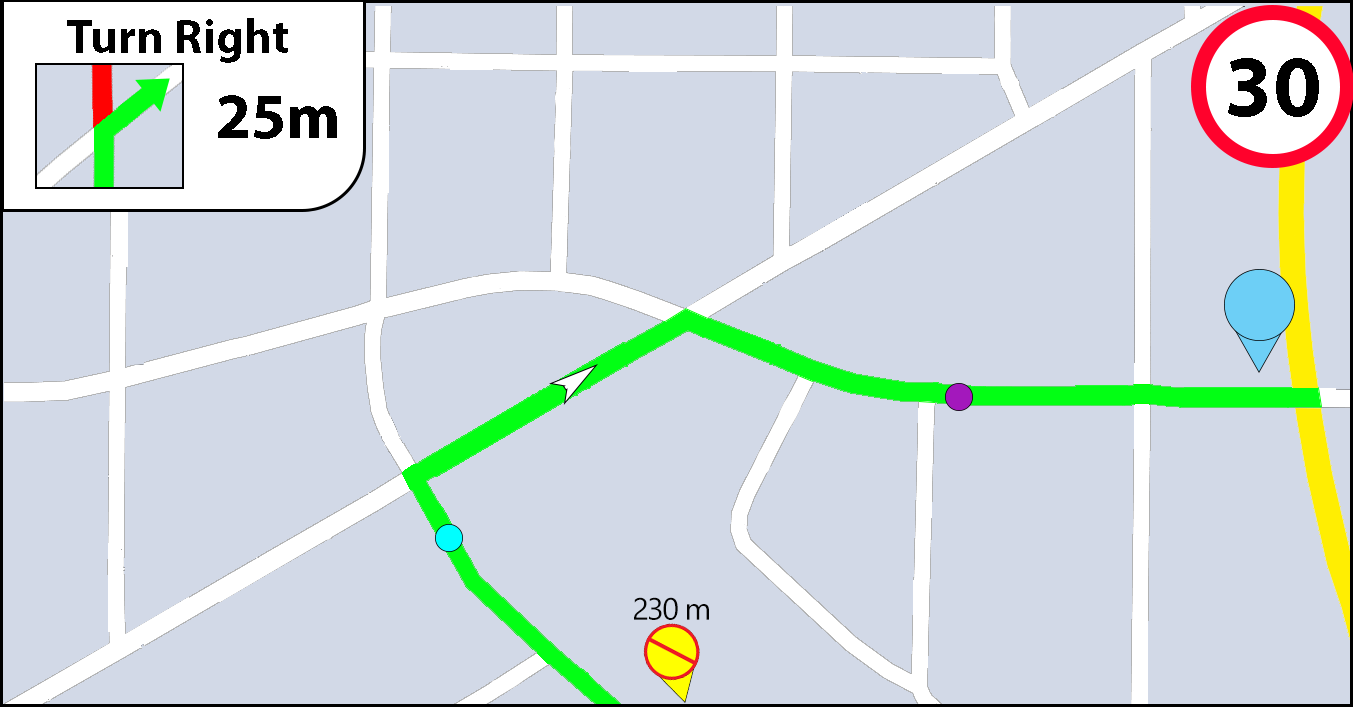
\includegraphics[scale=0.5]{convoy-map}
  \caption{Hi-Fi final design for navigation}\label{prototype-lofi-convoy}
\end{figure}


\subsection{Final design}\label{ssec:nav-final-design}

\subsection{Evaluation \& how it fits into whole system}\label{ssec:nav-evaluation}


%%%%%%%%%%%%%%
%
%	APP
%
%%%%%%%%%%%%%%
\section{Feature 2: App}\label{sec:app}

\subsection{Research --- Matt}\label{ssec:app-research}
Research and brainstorming were conducted in a cyclic manner to ensure that the latest technologies relevant to this sector of the automotive industry were taken into consideration. Extensive research revealed that most leading companies such as Jaguar, BMW and Tesla already offer multi-platform mobile apps that compliment their automobiles. Each of the above boasts at least one of the features that we intended to integrate into our systems such as remote control and seamless route porting from smartphone to car. From brainstorming through to coding the prototype, our focus was directed on how to improve on existing products and also integrate our novel features.
The research methods we used included a questionnaire, installing and using manufacturers apps on our mobile devices, browsing their websites and reading through papers and articles found through numerous searches on search engines. 

While browsing the existing apps that manufacturers offer, we have come across some flaws that  we were determined to get right in our final product. For example, \textit{BMW Connected}, their take on an app to compliment their most recent cars, excels in features like learning driving habits over time and facilitating safe communication with friends and family while still requiring a wired connection for simple features like transferring a route from the phone to the cars' navigation system and having a restricted range for remote functions such as lock, beep horn and switch lights. Flaws of similar magnitude con be found in \textit{Jaguar In-Control apps} and \textit{Mercedes Me}, which is reviewed as unusable or useless by most users.

We found that even where features are collectively good, they are often scattered over several apps, we intended for our customers to be able to download one app and be able to access all features from there while keeping it intuitive and user friendly.

Part of the second iteration of research involved looking into how useful different types of people find different features. This was achieved by polling friends and family of each of us, and therefore diversifying ethnicity, background and locations. We have then attached each to each of our features discussed in the brainstorming session to some personas for whom it would be relevant and this helped us decide how to prioritise our ideas.

\subsection{Brainstorming}\label{ssec:app-brainstorming} % Chris
When brainstorming ideas for the accompanying app for our car system, we considered both functional and non-functional requirements. We opened up a Google Doc so that we would all be able to contribute and follow along quickly since we all knew we had a lot of ideas for app integration features. One of the reasons that we all had so many ideas already was because we had already suggested certain ideas while planning features for the car's system previously.

We didn't rule out any ideas at this stage since even the most ridiculous ideas can spark inspiration for a more realistic and useful idea (``no idea's a bad idea''). Not ruling out ideas also kept our brainstorming phase moving quickly and meant that people were happy to go ahead with anything they thought of.

Once we couldn't come up with any more ideas for our initial brainstorm, we grouped each idea by features in a separate ``refined ideas'' document one by one after first discussing whether the idea was feasible and worth expanding upon. Once we had our completed refined and grouped ideas document, we were ready to start designing and researching technical details.

A section of our initial ideas brainstorming document can be seen in figure~\ref{initial-ideas} and a secion of our refined ideas can be seen in figure~\ref{refined-ideas}.

\begin{figure}[H]
  \centering
  \fbox{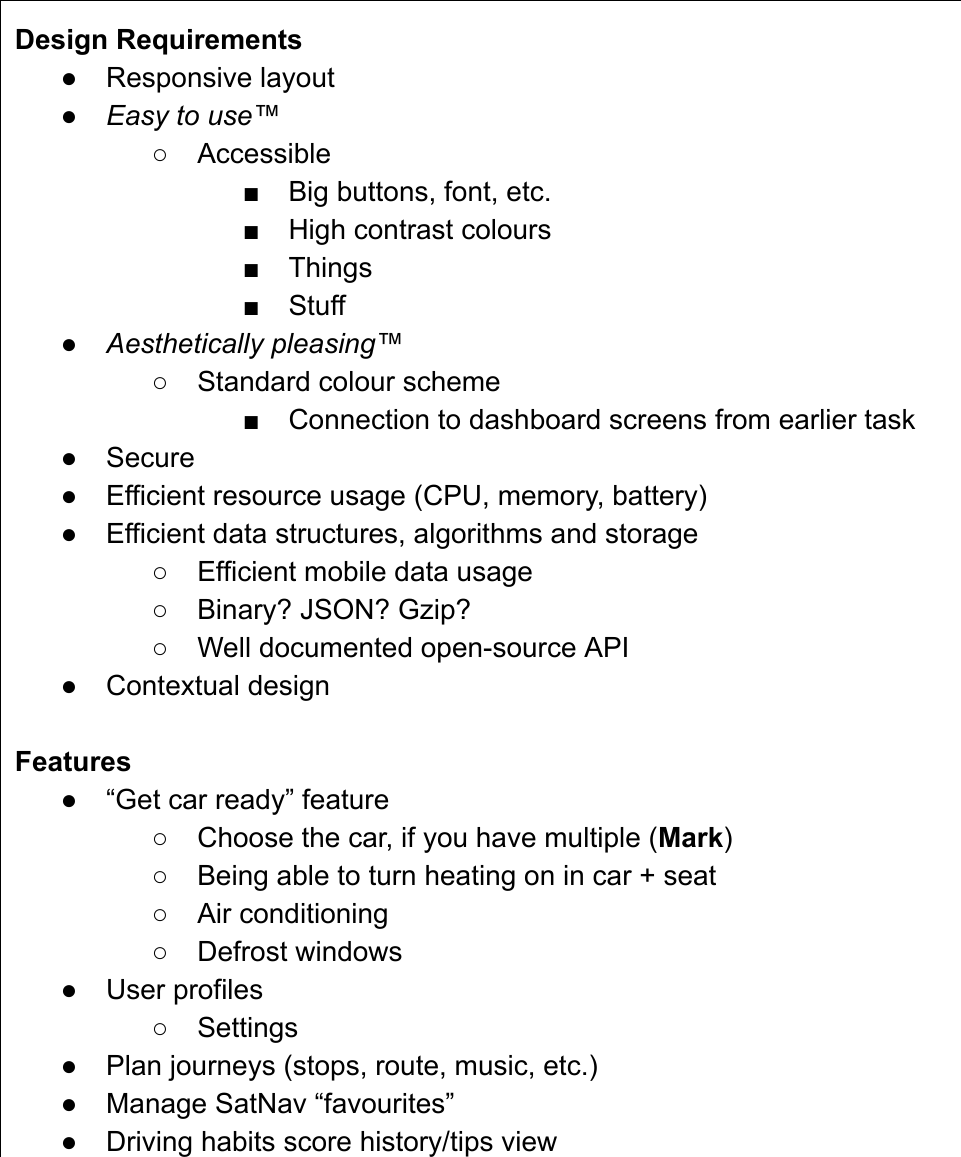
\includegraphics[scale=0.25]{initial-ideas}}
  \caption{Initial ideas brainstorming document.}\label{initial-ideas}
\end{figure}

\begin{figure}[H]
  \centering
  \fbox{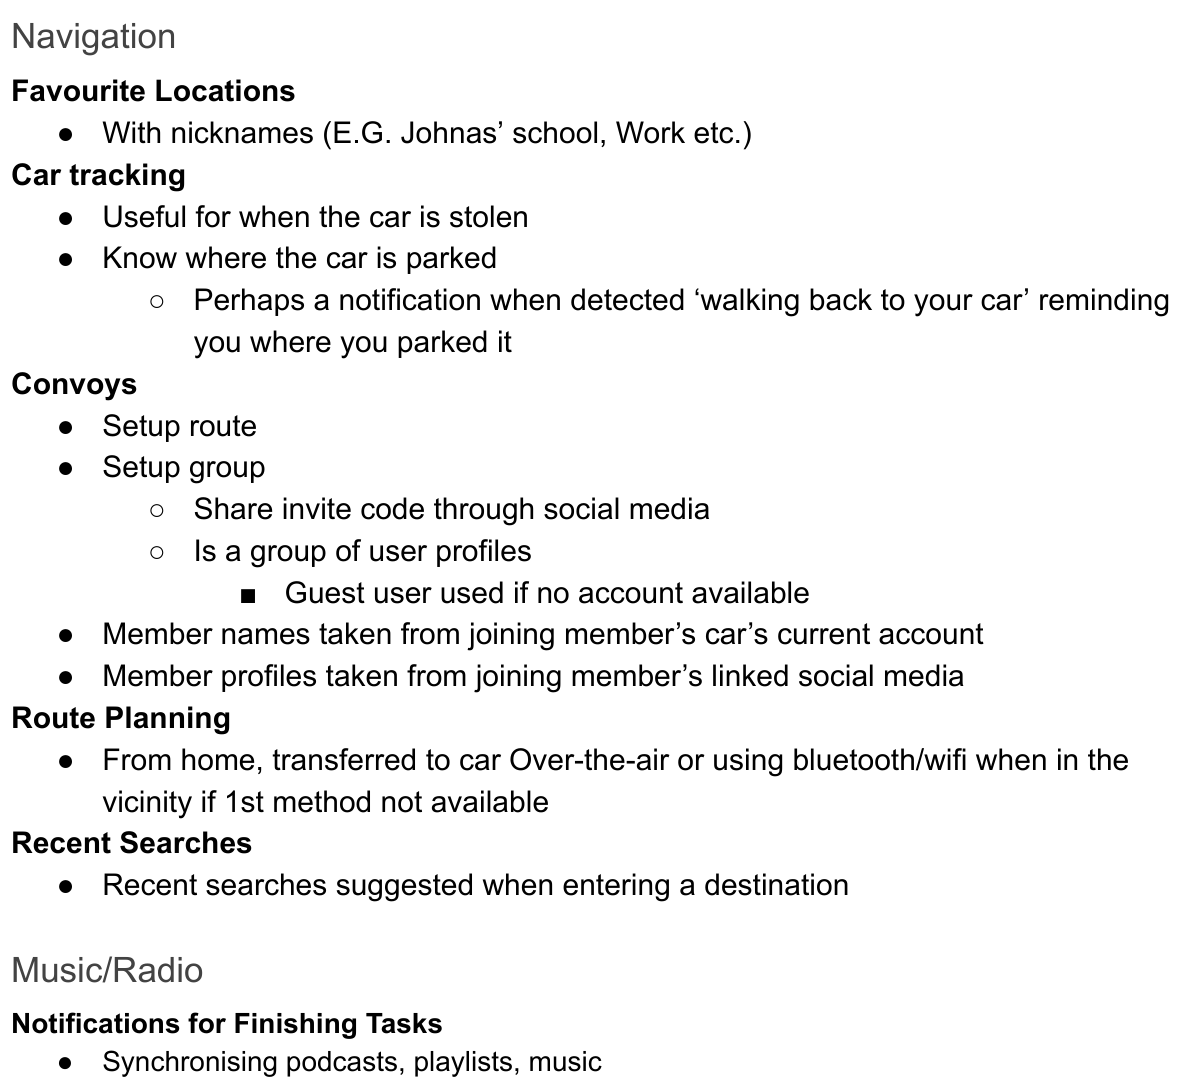
\includegraphics[scale=0.25]{refined-ideas}}
  \caption{Refined ideas document.}\label{refined-ideas}
\end{figure}

\subsection{Tech background}\label{ssec:app-tech} %Tyler
Many features of the app rely on communication with the car in order for them to work. These messages are sent between the phone to the car's central computing unit to be processed. Features which send instructions to the car to control the car's hardware have two different types of communication.

Firstly, instructions such as turn the heating on or toggling headlights will be a be on an on/off basis. For example setting the temperature to 20 degrees will keep it at that until it has changed.

Secondly, instruction-critical tasks such as remote controlling the car with the phone app, rapidly send instructions to the car to ensure the car is performing actions safely and as the user expects. For example, if a user is holding the steering wheel at a 45 degree angle, the associated instruction will be sent constantly and processed by the central computing unit until the user changes the rotation. If the phone would happen to lose connection and the instructions stop being received by the car, the car is stopped.

Features for controlling music within the car are communicated over Wi-Fi and Bluetooth. The local music library of the car is synced with the phone, and also there is a Spotify account linked to the drivers user profile. Which is logged in on the centre console.

All messages regarding the control of music with the app, are encapsulated within a JSON object. These messages will hold instructions such as play, pause and song requests. Song requests will contain music file names and the library they are stored in.
If music is from Spotify, then associated actions for controlling the Spotify account, which is logged in on the centre console are embedded within the message.

There is also the option to control the centre console Spotify account using Spotify's ``Spotify connect'' service. This allows you to control other Spotify devices on the same network. The Wi-Fi network of the car in this case.

Users can also view the car cameras live video feed on their phones through our app. This video stream will be dynamically re-encoded by the cars computing unit and then transmitted over RTSP (Real Time Streaming Protocol). This is to make best use of the connection of the car by adjusting the bitrate of video based on the available bandwidth from the car and to the client, whether they are connected via Wi-Fi or slow mobile data.
\begin{itemize}
  \item Data base
\end{itemize}

\subsection{Design choices \& argumentation}\label{ssec:app-design}
% While I put my name down for this, it's come to my attention that I'm probably not a great candidate for this section being that I wasn't present for a lot of the design choices for the app --- maybe this section is better written by somebody else -Lewis
\begin{itemize}
  \item QOC (to be made)
\end{itemize}

\subsection{Prototypes \& user testing}\label{ssec:app-prototypes-testing}
\begin{figure}[H]
  \centering
  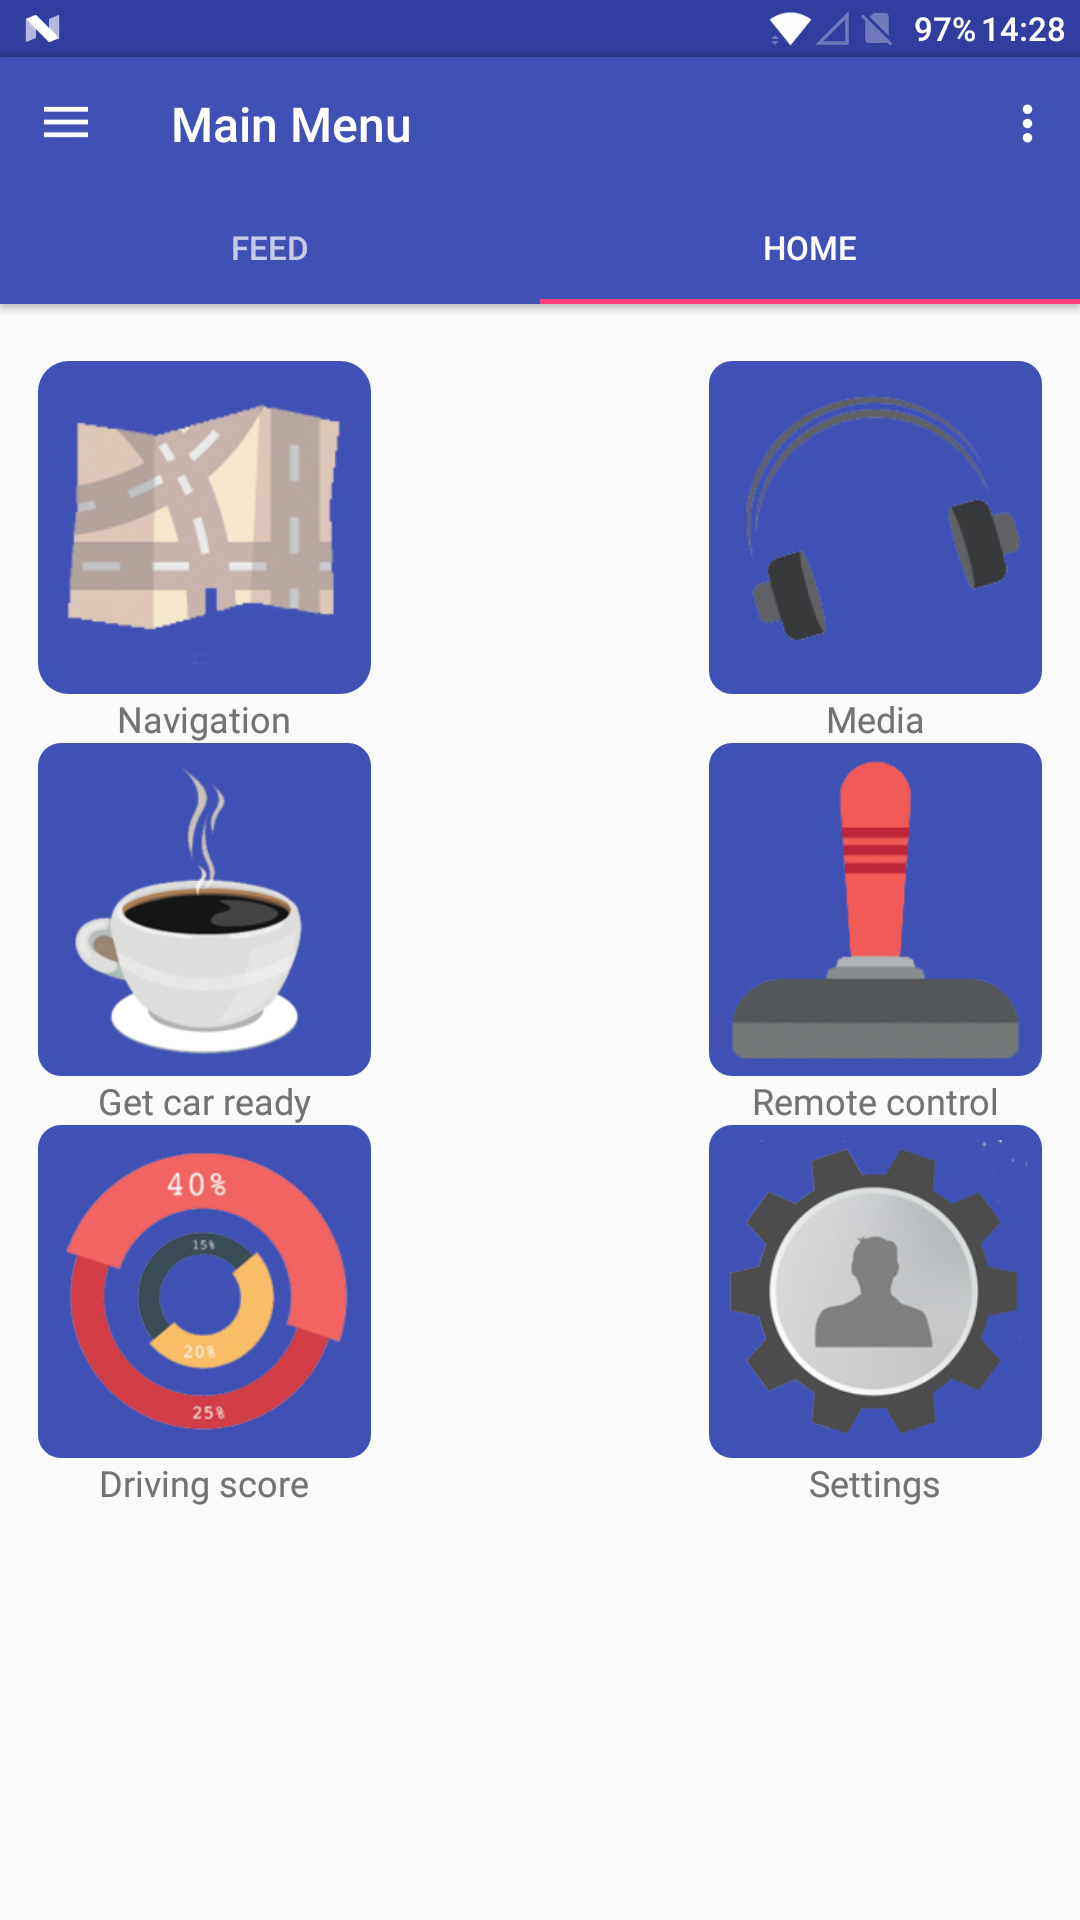
\includegraphics[scale=0.25]{main-menu}
  \caption{Hi-Fi prototype of app main menu.}\label{main-menu}
\end{figure}

\subsection{App Security}\label{ssec:app-security}
% Authentication via a phone built-in method as additional security 
% 2FA

\subsection{Final design}\label{ssec:app-final-design}

\subsection{Evaluation \& how it fits into whole system}\label{ssec:app-evaluation}

\section{Other areas}\label{sec:other}
Annotate slides on changes we would make going forwards

\includepdf[pages=1]{slides}
\includepdf[pages=2]{slides-annotated}
\includepdf[pages=6]{slides-annotated}

%\end{multicols}

\bibliographystyle{agsm}
\bibliography{references}

\end{document}

% vim: set tabstop=2 shiftwidth=2:
